\documentclass[12pt,oneside,a4paper,chapter=TITLE, english, french,	spanish, brazil]{abntex2-logatti}


\titulo{Caracterização das dimensões afetivas negativas em perfis de redes sociais por meio de Inteligência Artificial.}
\curso{Sistemas de Informação}
\autor{Guilherme Diego Albino Francisco}
\RG{40.741.310-8}
\local{Araraquara - SP}
\data{\MONTH\space / \the\year}
\orientador[Orientadora:]{Cristina Cibeli Vidotti Ivo de Medeiros}
\preambulo{Trabalho de Conclusão de Curso, apresentado às Faculdades Integradas de Araraquara, como requisito parcial para obtenção do título de Bacharel em }

\begin{document}

% Retira espaço extra obsoleto entre as frases.
\frenchspacing 

% ----------------------------------------------------------
% ELEMENTOS PRÉ-TEXTUAIS
% ----------------------------------------------------------
 \pretextual


\imprimircapa

\folhaderosto



\newcommand{\listofgraficosname}{Lista de Gráficos}
\newcommand{\graficoname}{Gráfico}
\newfloat[chapter]{grafico}{logr}{\graficoname}
\newlistof{listofgraficos}{logr}{\listofgraficosname}
\newlistentry{grafico}{logr}{0}

\counterwithout{grafico}{chapter}
\renewcommand{\cftgraficoname}{\graficoname\space}
\renewcommand*{\cftgraficoaftersnum}{\hfill--\hfill}


\pagebreak
\begin{dedicatoria}
 Este trabalho é dedicado a todos que um dia sonharam em melhorar a vida de alguém com grandes ou pequenos atos.
\end{dedicatoria}


\begin{agradecimentos}
Primeiramente gostaria de agradecer aos meus pais, minha irmã e a toda minha família pelo apoio nesses últimos anos. Todas as vezes que tranquei a faculdade ou troquei de curso e mesmo assim sempre acreditarem no meu potencial e me incentivaram. 

Gostaria de agradecer a todos os professores da Logatti. Em especial ao Fabio Fornazzari Papini que além de um excelente coordenador sempre foi um grande amigo e me deu grandes conselhos e orientação nessa caminhada profissional. 

Meu agradecimento mais que especial a minha orientadora Cristina Cibeli Vidotti Ivo de Medeiros, que me introduziu a Inteligência Artificial e sempre acredita em tudo o que me proponho a fazer por mais maluco que seja. 

Por último, porém de longe menos importante a todos os meus amigos, que sempre estiveram do meu lado me levando para frente, gostaria de nomear alguns nesse agradecimento. 

Jéssica Temporal e Leticia Portella me levaram a ter interesse por análise de dados e me ensinaram muito sobre o mesmo. 

João Daher e Mateus Freira que sempre me sedem um pouco do seu tempo para me passar algum conhecimento valioso de inteligência artificial. 

Alex Cortes e Tiago Correa que me ajudaram com toda a parte visual do projeto.

Por fim Jaqueline Alves que me ajudou demais com a parte de psicologia cuja a mesma não tinha conhecimento nenhum, foi graças a suas referências que pude tocar essa ideia.



\end{agradecimentos}


\begin{epigrafe}
“You don't understand anything until you learn it more than one way” – MINSKY,
marvin. Managing an Information Security and Privacy Awareness and Training
Program (2005)
\end{epigrafe}



% resumo em português
\setlength{\absparsep}{18pt} % ajusta o espaçamento dos parágrafos do resumo, espaço entre o resumo e as palavras-chave
% \begin{resumo}
%  Segundo a ABNT, o resumo deve ressaltar o
%  objetivo, o método, os resultados e as conclusões do documento. A ordem e a extensão
%  destes itens dependem do tipo de resumo (informativo ou indicativo) e do
%  tratamento que cada item recebe no documento original. O resumo deve ser
%  precedido da referência do documento, com exceção do resumo inserido no
%  próprio documento. (\ldots) As palavras-chave devem figurar logo abaixo do
%  resumo, antecedidas da expressão Palavras-chave:, separadas entre si por
%  ponto e finalizadas também por ponto.

%  \textbf{Palavras-chave}: latex. abntex. editoração de texto.
% \end{resumo}


% resumo em inglês
% \begin{resumo}[Abstract]
%  \begin{otherlanguage*}{english}
%    This is the english abstract. 

%    \textbf{Key-words}: latex. abntex. text editoration.
%  \end{otherlanguage*}
% \end{resumo}



% ---
% inserir lista de ilustrações
% ---
\pdfbookmark[0]{\listfigurename}{lof}
\listoffigures*
\cleardoublepage
% ---


% Lista de Gráficos
% \pdfbookmark[0]{\listofgraficosname}{log}
% \listofgraficos*
% \cleardoublepage

% ---
% inserir lista de tabelas
% ---
% \pdfbookmark[0]{\listtablename}{lot}
% \listoftables*
% \cleardoublepage
% ---

% Lista de Quadros
% \pdfbookmark[0]{\listofquadrosname}{loq}
% \listofquadros*
% \cleardoublepage


\begin{siglas}
  \item[APPA] Application to Process and Produce Analytic Data
  \item[IA] Inteligência Artificial
  \item[Tweet] Nome utilizado para postagem de um usuário no Twitter.
\end{siglas}


% ---
% inserir lista de símbolos
% ---
% \begin{simbolos}
%   \item[$ \Gamma $] Letra grega Gama
%   \item[$ \Lambda $] Lambda
%   \item[$ \zeta $] Letra grega minúscula zeta
%   \item[$ \in $] Pertence
% \end{simbolos}
% ---


% inserir o sumario
% ----
\pdfbookmark[0]{\contentsname}{toc}
\tableofcontents*
\cleardoublepage
% ---



% ----------------------------------------------------------
% ELEMENTOS TEXTUAIS
% ----------------------------------------------------------
\textual

\chapter*[Introdução]{Introdução}
Atualmente a saúde mental é um assunto cada vez mais recorrente e relevante na sociedade, porém os estudos sobre o assunto e seus transtornos já é algo antigo. Um dos marcos nos estudos sobre estados emocionais enfraquecidos foi quando Freud publicou sua obra “Luto e Melancolia”, que teve sua primeira publicação feita em 1916. A psicologia e a psiquiatria avançaram gradualmente no campo referente aos transtornos de humor, a comoção e relevância sobre o assunto teve impacto positivo na sociedade que se engajou mais em prol ao assunto, estabelecendo uma maior visibilidade ao tema.

Analisar um paciente com transtornos é uma tarefa cotidiana para um psicólogo ou psiquiatra. A forma com que as pessoas utilizam recursos como fala e escrita deixam traços que podem ser utilizados para analisar padrões emocionais e comportamentais. Cotidianamente, principalmente depois da ascensão das redes sociais, a quantidade de usuários interagindo cresceu e expressar-se publicamente se tornou mais simples.

Devido aos compartilhamentos em redes sociais, a quantidade de conteúdo disponível vem apenas crescendo, basta um rápido acesso a um perfil para mapear informações pessoais, sejam elas exatas como nome, idade, endereço e até familiares ou conteúdos mais abstratos como gostos musicais e literários. O ápice tecnológico citado, que começou aproximadamente no início da 2010, deu inicio a era dos dados. O dado organizado é capaz de se mutacionar em informações muitas vezes desejadas e necessárias para os usuários, esse potencial juntamente a vontade recente, gerada pelos avanços informática, de obter mais praticidade e facilidade no dia-a-dia, fez com que os dados se tornassem ainda mais valiosos. Empresas como Facebook, Google, Uber e Airbnb ganharam o mercado exatamente por conseguirem coletar os dados importantes e administrá-los em forma de soluções para seus usuários.

Aproveitando o momento, outras empresas começaram a utilizar dados públicos para criar ferramentas dedicadas a análise de mercado e tomada de decisão. A facilidade em mapear visitações, curtidas, compartilhamentos e até publicações opinando sobre algum produto ou serviço impactou o crescimento dessas ferramentas. Aplicar a mesma lógica para análise de perfil com a premissa de caracterizar se o usuário tem algum transtorno é mais complexo, porém factível.

Para mapear tais perfis seriam necessários especialistas analisando e gerando os dados desejados. O maior problema dessa abordagem, que se repete em quase todo processo que é automatizado, é o fator humano. A quantidade de profissionais não é escalável, ou seja, para que seja possível analisar mais dados seria necessário mais profissionais, e a quantidade de profissionais é finita. Além disso, a logística para registrar e manter os dados seria desgastante e não forneceria garantia de dados consistentes.

No entanto a automatização da análise desses profissionais apresenta algumas dificuldades devido o fato da maquina ser lógica. Nesse caso análise de dados abstratos como textos, só seriam possíveis com um forte mapeamento de propriedades como sentimento, sentido e palavras-chaves. O aprendizado de maquina e algoritmos de extração das propriedades citadas seriam de suma relevância, entretanto, uma vez que os dados fossem validados, e a maquina se tornasse capaz de replicar com certa assertividade a análise profissional, a quantidade de dados gerados seria maior e mais concisa devida a escalabilidade de uso de máquinas e a padronização gerada pela automatização do processo.

Partindo da premissa de que se é possível extrair informações necessárias, inferi-las em modelos psicológicos conceituados e a partir disso, obter-se dados condizentes para mensurar o impacto dos transtornos em um determinado perfil, a proposta deste trabalho é exatamente utilizar de dados públicos do Twitter, para coletar perfis e suas respectivas postagens recentes, seguido, em transformar essa base dados em uma base de conhecimento inserindo as propriedades citadas anteriormente, entre outras, com processamento e ajuda de profissionais, para isso além da mineração de dados será implementado um sistema capaz de recolher as análises de psicólogos e psiquiatras.

Será coletada uma base e os dados dos especialistas em primeiro momento serão simulados pelo autor, após isso a mesma base será utilizada para treinar uma IA afim de que ela seja capaz de replicar as análises dos profissionais, fazendo assim, com que a máquina seja capaz de identificar transtornos nos usuários.

Foi selecionado o paradigma funcional utilizada nas linguagens como Javascript, Python e GoLang para construção do \textit{softwares} e \textit{scripts} responsáveis pelo funcionamento do sistema. Além disso o banco utilizado será o MongoDB para armazenar o conjunto de dados pela alta \textit{performance} em leitura e indexação de dados.

\cleardoublepage
\chapter{SÍNTESE BIBLIOGRÁFICA}
\chapter{Revisão Bibliográfica}
A pesquisa proposta, assim como os temas abordados nela, é multidisciplinar. As próximas sessões abordarão tópicos necessários para o entendimento da posterior conclusão do projeto e suas abordagens.

Primeiramente será introduzido a \textbf{linguística} devido aos temas de analise de discurso, essencial para que seja possível analisar como as amostras se expressão em seus textos, e a introdução ao processamento de linguagem natural.

Em seguida, será necessário entender um pouco sobre \textbf{Psicologia}, dentro dela os tópicos traumas emocionais e modelos de mensuração que serão brevemente abordados devido ao cunho dessa pesquisa. Além disso, será introduzido ao conceito de Psicologia Cognitiva.

Os tópicos já explicados serão utilizados para fundamentarmos a \textbf{inteligência artificial}, nessa sessão tambem será apresentado o conceito base de IA com ênfase em aprendizado de máquina.

Por fim, será tratado o tema \textit{\textbf{Data Science}}, os tópicos relacionados a manipulação de dados, desde a mineração e gestão até a sua representação e organização.

\section{Linguística}
A gramática é composta por: um conjunto finito de letras que formam o chamado alfabeto e um conjunto de regras e normas. Utilizando das regras e do finito número de palavras formadas a partir das letras, é possível se expressar através de uma sentença. O estado representado por essa sentença pode variar de acordo com a regra aplicada. É impossível cobrir todos os estados com uma única regra pelo motivo de existirem números infinitos de sentenças a serem formadas \cite[13-25]{chomsky2002syntactic}. Essa capacidade de obter descrições de forma simplificada através da linguagem é a primeira área cognitiva do ser humano \cite[131]{putnam1975mind}.

No dia-a-dia, existem multiplos fatores que ajudam a entender o sentido de uma frase, porem, em uma máquina os mesmos fatores muitas vezes não se aplicam. Nessa sessão o enfoque é em introduzir alguns estudos fomentados pela linguística. Na inteligência artificial, o ato de juntar símbolos (padrões físicos) em expressões (estruturas) utilizando um conjunto de regras (processos), é considerado um sistema de símbolos físicos. Acredita-se que um sistema desse nesse formato possui os meios necessários e suficientes para realizar ações inteligentes de forma geral \cite[116]{newell1976ComputerSA}. Entretanto, o que foi escrito é diferente do que é compreendido, vide duplo sentidos, logo o contexto é necessário.

% sections
\subsection{Analise de Discurso}
No decorrer de um texto (que é algo concreto), pode-se caracterizar diversos níveis de geração de sentido.
A primeira formulação de sentido vem do discernimento de termos dentro de um contexto, esse nível é chamado de fundamental. Após distinguir esse primeiro sentido ele é aplicado pelo autor através de um sujeito fazendo com que a prosa tome uma direção, esse nível é chamado narrativo. Por fim, existe o nível discursivo, relacionado as escolhas de tempo, espaço, pessoa e figura durante a narrativa dos fundamentos, dando a essa narrativa um ponto de vista. Logo, o termo discurso é dado como um suporte abstrato por trás do texto, afim da concretização da sua ideia central \cite[13-17]{gregolin1995ad}.

A analise de discurso é, de forma sucinta, uma analise do que foi dito, de como foi dito e qual o sentido do que foi dito. As primeiras manifestações do assunto foram no século XX com autores russos que, além de isolar e definir elementos de uma linguagem poética queriam definir determinantes por trás do perfil artístico do escritor. O tempo fez com que a analise de discurso se desenvolvese e ramificasse em várias vertentes, uma delas a francesa, que apoia a possibilidade de automatizar essa analise por meio da informática. A área continua sendo um campo complexo e de contínuo estudo por trás das definições e metodologias para abordar e sustentar as novas unidades de analise. \cite[22]{souza2006ad}.

Os discursos se diferem de pessoa para pessoa devido ao nível discursivo, a necessidade de expressar um determinado sentido leva o autor a se colocar em um ponto de vista durante sua narrativa. Do contexto da pesquisa, entender o discurso do usuário para mapear o motivo do seu estado mental é um fator de total relevância para entender o estado dele. A pesquisa realizada por Modesto Leite \cite[134]{modesto2005adepre}, mostra em seus resultados que os discursos apresentados pelos pacientes fundamentavam o motivo psicológico do por que os mesmo teriam o transtorno. 

Partindo dos principio apresentados sobre um discurso, por mais que as palavras sejam localizadas, o ponto chave da discussão está em como um computador seria capaz de inferir o sentido da frase. Existem áreas, seguindo os campos multidiciplinares que envolvem linguitica e computação, responsáveis por garantir que o processamento dos textos gerará os resultados esperados.

\subsection{Processamento de Linguagem Natural}
Se entender palavras não significa entender o contexto, logo, se familiarizar com o ambiente e o momento afim de idealizar o que está sendo transmitido é algo necessário. Essa conexão entre elementos é tratada no estudo do \textit{connectivism}\footnote{Integração dos princípios de rede, caos, complexidade e teorias de auto-organização. Seu objetivo é entender decisões baseado nas mudanças de componentes fundamentais \cite{siemens2014connectivism}.}. De acordo com a linha de pensamento, estabelecida pelo estudo, os neurônios seriam os agentes cognitivos responsáveis por planejar, construir e representar essas informações que o cérebro humano recebe. Criar soluções para problemas pontuais que envolvam a língua que é utilizado no dia-a-dia se uma pessoa, essa é a definição por trás do Processamento de Linguagem Natural (PLN). Fornecer dados linguísticos que a maquina não é capaz de inferir, ou que seja necessário uma ajuda para seu melhor desempenho, é o ponto principal dessa área \cite{brandura1996, maria2015npl}.

Já que o PLN será inicialmente utilizado para análise de palavras-chaves e padrões, é necessário vislumbrar que será necessário um conjunto de regras a fim de melhorar uma determinada métrica durante o processo de aprendizagem. Para que isso seja possível, um conhecimento dentro da área de psicologia se torna altamente relevante.


\section{Psicologia}

A psicologia é, descrita como, a ciência da vida mental, capaz de analisando os desejos, sentimentos, razões, sentimentos, decisões entre outras faculdades mentais entender o posicionamento e o estado emocional do ser. Entender o nosso estado e como isso impacta em a vida é o grande desafio da área \cite[4-8]{william1890principles}.

Nossa pesquisa utiliza da psicologia em dois pontos distintos, porem, interligados. A primeira delas é o envolvimento da psicologia com a depressão, em segundo a participação da área da psicologia cognitiva na evolução da Inteligencia Artificial. Ambos os pontos se interligam ao se questionar o motivos de alguem ter depressão, ou o quão plausivel é o mapeamento disso através de técnicas desenvolvidas dentro da área nos ultimos anos.

% sections
\subsection{Depressão}
Desanimo, perca de interesse, inibição e bloqueio de sentimentos são alguns sintomas exibidos por pessoas melancólicas \cite[276]{freud}. A \textbf{melancolia} seria uma condição maléfica de enfraquecimento da sáude mental de um ser. Partindo do principio de Fairbain onde o ser humano busca por gratificação, a não gratificação poderia ser o motivo de um estado melancólico.

A \textbf{depressão} é uma forma atenuada de melancolia \cite{roudinesco2000}. Classificada como \textbf{transtorno de humor}, diferente de outras variações mais regulares de humor, pode causar grandes danos a vida cotidiana uma vez que, por definição, altera a percepção de si mesmo maximizando o peso dos seus problemas diante de sua própria pespectiva. Por tais motivos, a melancolia e a depressão compartilham de sintomas similares, entretando, a dinamica de suas origens, relações e concepções podem criar diversas perspectivas o que leva ao ponto de como se pode medir algo tão abstrado. \cite{}

\subsection{Ansiedade}

\subsection{Escala Depressão, Ansiedade e Stress}
Adotando um modelo dividido em 3 sub-escalas a \textbf{Escala de Depressão, Ansiedade e Stress} ou \textbf{EADS} foi proposta na premissa de uma maior assertividade na analise das dimensões afetivas negativas, uma vez que existiam outras pesquisas com proposta similar como o \textit{ Beck Anxiety Inventory} (BAI) e \textit{Beck Depression Inventory} (BDI). As diferenças entre essas escalas são: sua execução, o fator de correlação das sub-escalas propostas pelo EADS e o inventário de Stress introduzido durante o estudo (como mencionado na sessão anterior).  

A EADS completa é composta de 42 itens, por fins de facilitar a geração de dados iremos usar o modelo de 21 itens, que são divididos igualmente entre as escalas e mesmo que um deles pertença a uma escala ele pode ter correlação com alguma outra. Esses itens são afirmações que podem ser respondidas por números de 1 a 4 que representam desde "não se aplica a mim" até "se aplicou a mim na maior parte das vezes" e no final serão somados a fim de gerar um resultado para a sub-escala, os maiores valores representam as dimensões mais negativas \cite{lovibond1995structure, ribeiro2004contribuiccao}.

Diferente da proposta de auto avaliação ou avaliação mediada\footnote{Nesses casos os usuários são responsáveis por responder as perguntas por si mesmos ou por meio de um mediador que ira preencher o formulário.}, como é proposta pela EADS,  uma das premissas da pesquisa é inferir os resultados das escalas utilizando textos cotidianos de uma amostra em rede social. Isso nos leva a entender os conceitos cognitivos por trás da psicologia que levaram os autores a propor suas escalas e pesquisas.



\subsection{Psicologia Cognitiva}
Dentro da Psicologia existe um ramo cujo o objetivo é entender a capacidade animal de pensar, memorizar, perceber e no caso humano utilizar um dialeto (linguagem), essa área de estudo ficou conhecida como psicologia cognitiva.

O ato de entender os procedimentos cognitivos adotados pelo ser humano se tornou mais relevante após a proposta da criação de uma inteligência artificial. O questionamento de como uma decisão poderia gerar, afetar ou cancelar uma cadeia de eventos, seja ela durante um pensamento ou uma ação, partindo da capacidade humana de realizar múltiplas tarefas, algumas delas complexas como interpretar linguagens com tantas divergências, fez com que em 1958\cite[4-7]{broadbent1958perception} surgisse o primeiro modelo psicológico que propunha um fluxo similar ao processamento de informações de um computador.

As técnicas experimentais, como os modelos psicológicos, impactaram toda a área interdisciplinar das ciencias cognitivas. Novas abordagens como a junção de modelos criados em computação para IA e técnicas experimentais da psicologia foram criadas a fim do entendimento da mente humana. Durante a criação do \textit{General Problem Solver}, por exemplo, Newell e Simon propuseram não só a implementação de algoritmos descritos por antigos estudiosos afim de resolver um série de problemas, mas também, entender como a maquina estava realizando isso, assim, seria possível uma comparação com a mente humana \cite{newell1961gps, russell2003artificial}.

Nessa pesquisa, a psicologia cognitiva terá um grande impacto em entender como as amostras que contem ou não sintomas causados pelas dimensões afetivas negativas se comportam e pensam. Esse entendimento é essencial para o mapeamento dos atributos que serão processados pela IA afim de gerar os modelos para predição em dados ainda não analisados. Além disso, a psicologia cognitiva faz parte de todo o processo qualitativo de criação devido a ser um dos vários campos que compões a multidisciplinaridade dentro da IA.

\section{Inteligencia Artificial}

Inteligência é, por definição, uma coleção sistemática de habilidades e funções com objetivo de processar diferentes tipos de informações de diversas maneiras \cite[49]{guilford1982cognitive}. Simular essa "coleção sistemática de habilidades e funções", tais como reconhecer formatos, tragetórias, sinais, deduzir proposições entre outras, afim de criar entidades inteligentes é o foco da inteligencia artificial \cite[1]{russell2003artificial}. Desde que a inteligencia artificial passou a ser um campo de estudo a quantidade de abordagens apresentadas por diversos pesquisadores afim de construir uma máquina inteligente apenas aumentou. Esses métodos se auto-contribuiram até levar a IA para seu estado atual. \cite[2]{russell2003artificial}.
\section{Ciência por tras dos dados}
Como um ser humano, os dados têm seu ciclo de vida, esse ciclo pode alterar-se dependendo de sua finalidade dentro da aplicação. O nosso tema e nosso objetivo é coberto por uma matéria, já antiga, nomeada \textbf{KDD} ou \textbf{\textit{Knowledge Discovery in Database}}, embaixo dela existem varias subclasses como mineração de dados, analise de dados, probabilidade e até mesmo IA. A KDD se justifica pela sua metodologia de manipulação de dados afim de extrair o conhecimento almejado de um base. Se observar o fluxo descrito na \ref{fig:kdd}, pode-se notar que uma cadeia de eventos como: seleção, pré-processamento, mutação, mineração e interpretação. Esses eventos geram novos estados para o dado, e os moldam focando o objetivo de retirar o conhecimento pela interpretação no final do processo.

\begin{figure}[H]
    \centering
    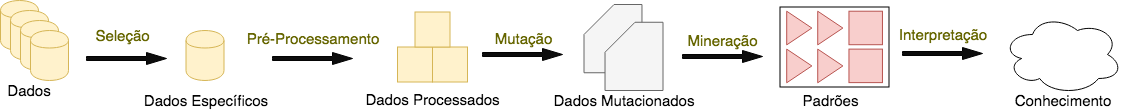
\includegraphics[width=.8\textwidth]{imagens/kdd.png}
    \caption{Representação da metodologia defendida pela KDD. Fonte: o autor.}
    \label{fig:kdd}
\end{figure}

Com o passar do tempo, vários novas abordagens surgiram para tratar dados, e essa massa de pesquisas e definições deu-se por bagunçar um pouco a nomenclaturas e definições que estão atrelados a \textbf{ciência por traz dos dados}. Para evitar confusões as definições apresentadas nessa sessão serão sucintas e tem como objetivo futuros tópicos e discussões apresentados durante os resultados dessa pesquisa. Devido a grande divergência, ocorrido pela disseminação rápida e conturbada de algumas termologias, sobre os temas abordados, serão seguidas as seguintes referencias \cite{laender2002brief, fayyad1996kdd, hand2007principles}.

\subsection{Extração de Dados}
A extração, é o ato de obter dados em massa de fontes externas, como \textit{websites} e \textit{apis}\footnote{A sigla API vem de \textit{Application Programming Interface} e é um interface que permite outras aplicações utilizarem de seus recursos e funcionalidades. Dentro do universo \textit{web}, o termo API é utilizado para descrever um conjunto de rotas que podem ser utilizados para acessar recursos de um aplicação online.}. Esse passo ocorre antes do passo descrito pela KDD como seleção. Conhecido pelo termo inglês \textit{data extraction}, tem sua relevância ao ser a primeira etapa para construir uma base de conhecimento.


\subsection{Seleção de Dados}
O ato de selecionar os dados com enfoque no conhecimento que você deseja obter deles afim de gerar um conjunto de dados especifico é também conhecido como \textit{\textbf{data collection}}, durante o processo do KDD é o primeiro passo responsável por gerar um amostra mais focada no problema.

\subsection{Mineração de Dados}
Nessa subseção propõe-se que seja dissertado sobre os processos do KDD a partir da seleção até a interpretação. Vale ressaltar que para obter conhecimento não é necessário uma IA, sistemas de tomada de decisão trabalham com probabilidade matemática sob dados exatos, o que em muitos casos, já seria o suficiente para obter a informação do dado. Entretanto, o foco da pesquisa se baseia na implementação de um sistema inteligente e isso inclina essa explicação para o fato de: o aprendizado de máquina é uma das possíveis formas de se minerar um dado.

A mineração de dados ou popularmente conhecida como \textit{data mining}, baseia-se em retirar os valores mais relevantes e valiosos para se inferir um conhecimento. Os demais passos como pré-processamento e mutação se assemelham a alguns processos citados anteriormente como a redução dimensional ou ainda a engenharia de atributos.


\subsection{Analise de Dados}
E finalmente, a analise. O passo descrito como interpretação no KDD se refere a entender os dados de saída vindos da mineração afim de afirmar ou descarta hipóteses, com isso é possível refinar o processo e explorar novas possibilidades. Uma das palavras que hoje se tornaram popular dentro dá área é o \textit{data storytelling}, ou, o ato do dado de contar uma história. Abordar a hipótese de maneira empírica e demonstrar a veracidade dela discutindo abordagem e algoritmos gerados é um dos objetivos dessa área.






\cleardoublepage
\chapter{MATERIAIS E MÉTODOS}
O objetivo da pesquisa é caracterizar dimensões afetivas negativas em perfis do twitter localizando pontos comuns entre usúarios portadores de afetividades negativas (stress, ansiedade e depressão) de mesmo nível. Esse tipo de processo se asemelha com a aprendizagem não supervisionada, logo, antes dessa etapa é necessário mapearmos atributos, sendo assim, é necessário a identificação de usúarios com dimensões afetivas negativas em primeiro momento.

Como observado, existem vários passos para conclusão desse projeto, abertamente estrutura de processamento contára com um processo de mineração e dois processos de inteligencia artificial afim de gerar dois modelos lógicos. O primeiro modelo responsavel por inferir valores da EADS em um perfil, e o segundo, de predizer, a partir de dados do perfil, a probabilidade de existir um determinado nível de afetividade utilizando dados do perfil.

O projeto em geral tem alguns outros pontos sociais envolvidos, que assim, tornam a área de atuação da pesquisa um pouco mais ampla, entretando nenhum desses pontos, exceto a utilização de profissionais capacidados para geração de alguns atributos na base da pesquisa, impactam diretamentamente a \textit{performance} e por isso não serão detalhados. Logo essa documentação é voltada unicamente ao sistema que será desenvolvido.

Pode-se observar na figura \ref{fig:tecnologias}, o sistema é divido em dois núcleos, o Dumont responsável por minerar e gerar toda a base de dados, e o 14BIS que será responsavel pelas Inteligencias Artificias. O aparente terceiro núcleo, na realidade, é simplesmente um banco de dados embutido gerado pelo APPA (ferramenta de administração de mineração de dados) dentro do Dumont e que será consumido pelo 14BIS posteriormente.

\begin{figure}
    \centering
    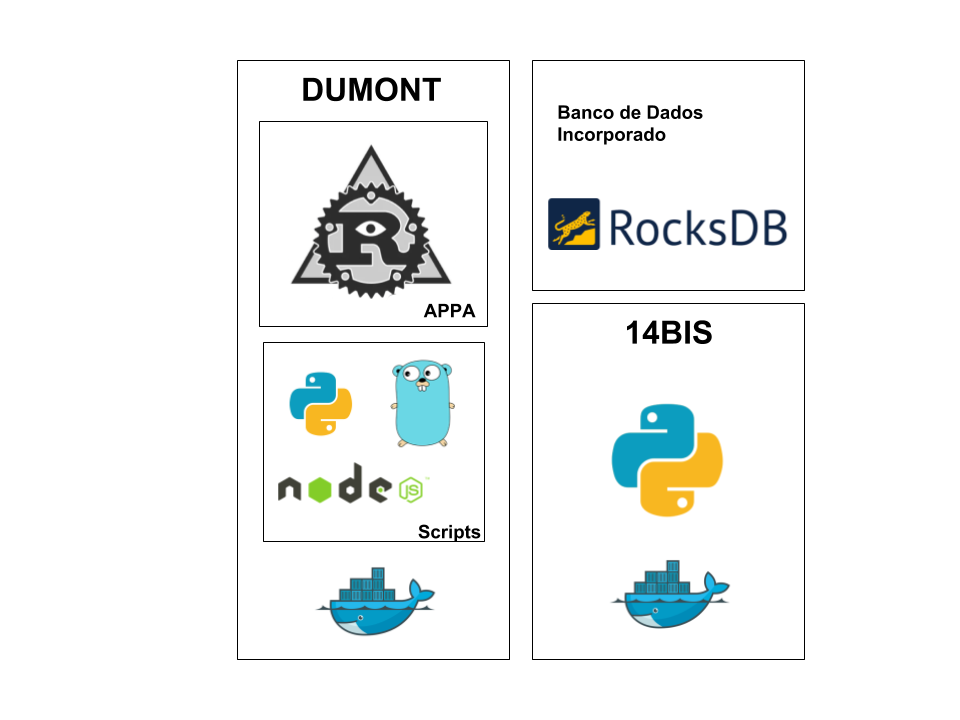
\includegraphics[width=.8\textwidth]{imagens/tecnologias.png}
    \caption{Desenho apresentando os núcleos do projeto}
    \label{fig:tecnologias}
\end{figure}

Existem basicamente 5 técnologias que estão sendo utilizadas nesse projeto:
\begin{itemize}
 \item Rust: Rust é uma linguagem altamente performatica, preza por custo zero em abstração, atua com excelencia em processamento paralelo e seu modelo de alocação de memória evita \textit{dataraces}\footnote{O termo \textit{datarace} traduzido abertamente como corrida de dados é um termo muito utilizado em processamento paralelo e envolve a tentativa de uso de uma alocação de memória por diferentes partes do sistema em um mesmo periodo de tempo}.
 \item Python: É a linguagem atual mais utilizada no mundo de Aprendizado de Máquina, sua simplicidade ja á torna simples de usar, porem, a quantidade de materiais, bibliotecas e artigos sobre PLN e Aprendizado de Máquina á tornam a principal linguagem nesse projeto.
 \item Node/Javascript: Node é o interpretador que permite com que seja possivel executar o Javascript (linguagem originalmente de navegar no servidor). A linguagem tem um grande ganho com integrações e será utilizada para consumir recursos vindos de APIs.
 \item Go: Asemelha-se muito com Rust, porem, tem um ambiente menos burocratico devido a seus diferentes objetivos. Go será a escolha para qualquer processo que não envolva API ou PLN.
 \item RocksDB: O RocksDB é um banco não relacionado, estrutura é baseada em duas \textit{strings} uma sendo chave e a segunda sendo um valor relacionado a essa chave. Bancos não relacionais tendem a ter leitura mais rápida que bancos relacionais, a estrutura do Rocks é baseada em logs e escrito em baixo nivel o que permite sua escrita ser tão rápida quanto sua leitura.
 \item Docker: Docker é uma ferramenta para infra-estrutura, será utilizado para rodar a aplicação em containers e facilitar o \textit{deploy}\footnote{Vindo do termo em inglês "lançar" é utilizado para o ato de colocar uma aplicação em ambiente de produção}.
\end{itemize}

Existirá uma sessão explicando o funcionamento do APPA, e como serão desenvolvidos os scripts que ele ira gerenciar, tanto quanto a parte explicativa sobre a Inteligencia Artificial, logo, nessa introdução os casos de uso serão tratados de forma sucinta. Se observar a figura \ref{fig:tcc_caso_de_uso}, notara que o Dumont ira utilizar da API do twitter para coletar dados públicos, posteriormente esses dados serão processados e mutacionados a fim de gerar uma base de dados, por final essa base dados será salva em um banco embutido. Tanto o Dumont quanto o 14BIS irão consumir os dados salvos, porem é responsabilidade do 14BIS consumi-los a fim de treinar as IAs desse projeto para gerar os modelos lógicos.

\begin{figure}
    \centering
    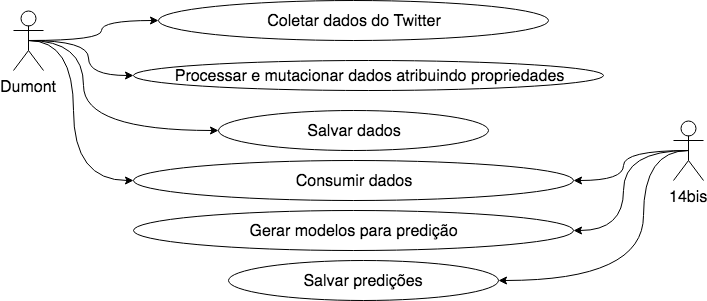
\includegraphics[width=.8\textwidth]{imagens/tcc_caso_de_uso.png}
    \caption{Diagrama de caso de uso do sistema}
    \label{fig:tcc_caso_de_uso}
\end{figure}

Para melhor entendimento a documentação será dividida em núcleos teóricos e práticos. Primeiramente será dado toda a descrição teórica sobre a escolha de atributos, e funcionamento das ferramentas que serão utilizadas no processo. Em seguida será detalhado os núcleos mais práticos como a coleta e mineração, onde alem de explicar como rodar o Dumont, tambem serão explicados como e por que foram construidas essas partes do sistema. Como ja dito, a primeira etapa se consiste em entender alguns dos atributos utilizados aqui.

\section{Engenharia de Atributos}
A escolha dos atributos, também intitulada popularmente como \textit{feature engineering}, é o ato mais importante durante a mineração de dados, por que é através desses atributos que as maquinas irão aprender. É válido destacar que essa sessão serve apenas para introduzir a razão dos atributos, seu detalhamento será dado durante a sua implementação.

O primeiro atributo relevante aqui é o sentimento. Já que será abordado dimensões afetivas negativas, o sentimento expressado por uma frase tem um grande impacto como atributo. Entretanto, o sentido em uma frase pode ser mais fácil de ser extraído em textos concisos, ou seja, normalizar os textos é necessário.

Um dos atributos utilizados aqui será o texto normalizado, para isso será utilizado o \textit{spacy}, uma biblioteca Python para remover palavras que oferecem apenas ruídos ao resultado. Além disso, também será tirada a arvore sintática, para que seja possível estabelecer padrões de discurso na IA, ou então, reconhecer certas palavras presentes em demais analises.

Uma vez observado os nossos atributos, seria necessário erguer um sistema capaz de realizar tarefas e persistir esses dados em algum banco de dados. Porém, será utilizado nessa pesquisa uma ferramenta para gerenciar tais tarefas.

\section{\textit{Application to Process and Produce Analytic Data (APPA)}}

Definir uma boa base de dados é o ponto mais critico durante a criação de uma inteligência supervisionada. O \textit{Application to Process and Produce Analytic Data} (APPA), ou, Aplicação para Processamento e Produção de Dados Analíticos, é um ferramenta criada capaz cadastrar tarefas, em qualquer linguagem e utilizar delas para coletar e processar esses dados afim de gerar uma base de conhecimento.

Explicando com mais detalhes, a figura \ref{fig:appa_eng} mostra o funcionamento da ferramenta. Existe uma arquivo chamado \textit{config.yml} que tem mapeado todas as tarefas e entidades de processamento. Essas tarefas podem ser escritas em qualquer linguagem de programação e algumas delas podem ser responsáveis por coletar dados, os scripts que são escritos com intuito de retornar dados para processamento são chamados coletores.

\begin{figure}
    \centering
    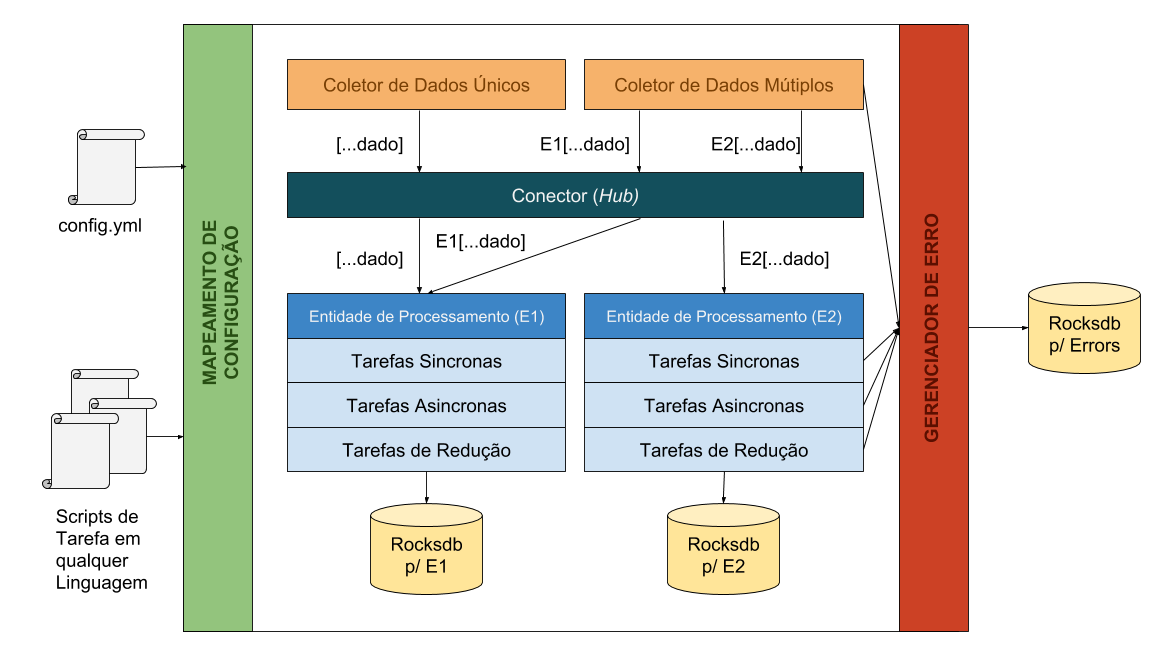
\includegraphics[width=.8\textwidth]{imagens/appa_eng.png}
    \caption{Diagrama demonstrando o funcionamento da ferramenta APPA}
    \label{fig:appa_eng}
\end{figure}

Um dado emitido por um coletor é marcado ou não por uma \textit{tag}, ou marcação, essa responsável por creditar qual coletor será responsável por processar. Por padrão um dado enviado sem destino é marcado com o simbolo \textit{underline}. Toda tarefa dentro do APPA é considerada uma tarefa com múltiplas saídas, logo, é possível enviar dados em lotes e tempo real para que o APPA processe dentro das entidades. 

Entidades de processamento, por sua vez, são compostas por coletores e tarefas de processamento. As tarefas de processamento podem ser síncronas ou assíncronas, ambas executam individualmente por unidade de dado, algo similar a uma linha de dados de um banco, a diferença é seu formato de execução, como o próprio nome fala as tarefas assíncronas não respeitam ordem de execução e são executadas paralelamente pelo processador. Alem disso existem as redutoras e/ou mapeadoras, consumiram todo o banco gerado após a execução das tarefas síncronas e assíncronas e retornara um novo estado para o banco total. Cada entidade gera seus dados em um banco incorporado isolado para os dados processados por elas.

Diferente de outras ferramentas, o processo de mineração nunca é interrompido. Qualquer erro que aconteça na aplicação é gerenciado por uma camada e registrado em um banco de erros, após isso o processamento segue para os demais dados.

\section{Tarefas de Processamento}
Como explicado, o APPA ira gerenciar nossas tarefas de processamento, ja foi abordado também alguns atributos que serão necessários para 14BIS executar os modelos lógicos. Tendo isso em vista é necessário que seja implementado \textit{scripts} de mineração e pré-processamento para que a base de dados de dados do projeto tenha a estrutura necessária para que as IAs possam agir.

Essa sessão tem como objetivo detalhar os atributos e \textit{scripts} criados para gerar-los. Além disso em alguns casos, onde são utilizados recursos externos como APIs, será detalhado a configuração necessária.

É importante ressaltar que todo o projeto é \textit{Open Source}, conhecidos como projeto de código aberto, e todo o código criado para esse projeto pode ser encontrado na plataforma de versionamento do GitHub\footnote{\url{https://github.com/getdumont}}.

Antes de iniciarmos as explicações é necessário que para reprodução dessa pesquisa você tenha inicialmente o Docker\footnote{\url{https://www.docker.com/}} instalado. Caso deseje executar as tarefas individualmente, como será citado aqui, é necessário que você tenha instalado na sua máquina o Python 3.6\footnote{\url{https://www.python.org/downloads/release/python-360/}} e o NodeJS 9.11\footnote{\url{https://nodejs.org/en/blog/release/v9.11.1/}}. Vale lembrar que todo código aqui demonstrado foi escrito, executado e testado em um sistema operacional com base Unix, logo a portabilidade com Windows não é garantida.

Uma vez com as ferramentas instaladas no sistema operacional, torna-se possível a reprodução dessa pesquisa. A primeira etapa como já discursada até então se refere a coleta de dados.

\subsection{Tarefa de Coleta}
A coleta será feita utilizando a API publica do twitter, o link para a documentação é \url{https://developer.twitter.com/en/docs}. Será trabalhado no projeto duas entidades: Tweet e Usuário. O tweet é a entidade que representa a publicação do usuário, enquanto o usuário contém informações necessárias sobre o seu perfil.

Para que seja possível acessar a API é necessário criar uma conta de desenvolvimento e gerar o \textit{token} de acesso\footnote{\url{https://apps.twitter.com/app/new}}. Com a chave em mãos é possível replicar o arquivo /collector/client/.env\_sample dentro do projeto Dumont para /collector/client/.env, e conforme demonstrado na figura \ref{fig:twitteropts}, completar os campos necessários.

Para rodar basta executar o comando \textit{node collector/twitter.js}, e verá a saída de dados. Existem duas observações relevantes a serem feitas nessa etapa:
\begin{itemize}
  \item !AppaTag(tweet) e !AppaTag(user): Se notar, algumas linhas começarão com essas duas anotações, são essas anotações que serão responsáveis por fazer com que o APPA identifique qual entidade de processamento será responsável por processar cada tipo de dado.
  \item Dados de Emoji: É possível notar que alguns dados mapeados não existem na API do Twitter. Como observado, um dos problemas durante a mineração de dados é o uso de \textit{emojis} em textos, já citado também, é possível algumas tarefas de pré-processamento serem executadas durante a própria coleta. Sabendo que emojis podem expressar sentimentos \cite{novak2015sentiment}, e que armazenar e tratar esse dado poderia ser relevante na hora de confirmar sentimento em frases, o autor também criou a biblioteca \textit{Emojinator}\footnote{https://github.com/getdumont/emojinator}, além do texto tradado, também será obtida informações do \textit{emojis} utilizados no meio do texto.
\end{itemize}

\begin{figure}
    \centering
    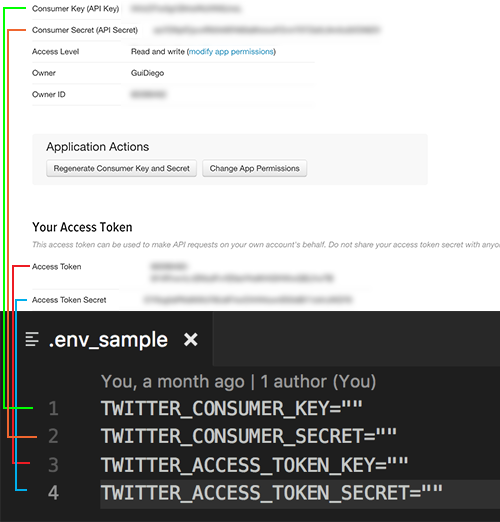
\includegraphics[width=.8\textwidth]{imagens/twitteropts.png}
    \caption{Imagem demonstrando onde cada chave deve ser inserida no código}
    \label{fig:twitteropts}
\end{figure}

Uma vez configurado o coletor, ainda é necessário entender e configurar as outras tarefas para que o APPA funcione apropriadamente, logo, é necessário entender como essas entidades ficarão no final e quais as tarefas que realizarão essa manipulação.



% \chapter{RESULTADOS, ANÁLISE E DISCUSSÃO}

% \chapter*[Considerações Finais]{Considerações Finais}





% ----------------------------------------------------------
% ELEMENTOS PÓS-TEXTUAIS
% ----------------------------------------------------------
\postextual
% ----------------------------------------------------------

% ----------------------------------------------------------
% Referências bibliográficas
% ----------------------------------------------------------

\bibliography{references}


% Inicia os apêndices
% \begin{apendicesenv}


% \partapendices % Imprime uma página indicando o início dos apêndices


% \chapter{Quisque libero justo}







% \end{apendicesenv}



% ----------------------------------------------------------
% Anexos
% ----------------------------------------------------------

% ---
% Inicia os anexos 
% ---
% \begin{anexosenv}


% \partanexos  % Imprime uma página indicando o início dos anexos

% ----
% \chapter{Primeiro}

% Este anexo é sobre como se pode ficar rico. Para ficar rico...





% \end{anexosenv}


\end{document}
